\title{Kirchhoff's Rules}
\author{Jordan C. Hanson}
\date{\today}
\documentclass[12pt]{article}
\usepackage[margin=2cm]{geometry}
\usepackage{amsmath,mathtools}
\usepackage{graphicx}

\begin{document}
\maketitle

\begin{abstract}
Kirchhoff's Rules will help you to understand more complex DC circuits by applying charge and energy conservation.
\end{abstract}

\section{A Complex Circuit}

Consider Fig. \ref{fig:circuit1}.  There are two power sources, a battery providing 15 V and a battery providing 10 V.  There are three currents, and they are labeled $I_1$, $I_2$, and $I_3$, and given directions.  Positve current flows in the direction of the arrows, but our results for the currents can be negative.

\begin{figure}[hb]
\centering
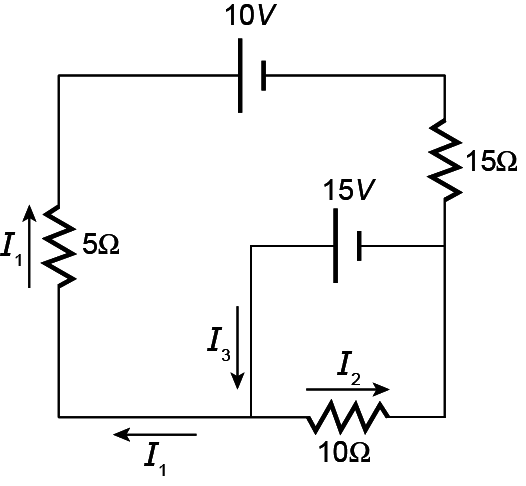
\includegraphics[width=0.35\textwidth]{figures/circuit_complex.png}
\caption{\label{fig:circuit1} A circuit with three currents and two batteries.}
\end{figure}

\section{Kirchhoff's Rule for Current Junctions}

Consider Fig. \ref{fig:circuit1}, at the point at the bottom where $I_3$ splits into $I_1$ and $I_2$.  The first of Kirchhoff's Rules is the following: \\

\textit{Since charge is conserved, the total current flowing into a junction must equal the total current flowing out of the junction.} \\

This implies that

\begin{equation}
\boxed{I_3 = I_1 + I_2} \label{eq:current}
\end{equation}

Can you identify the other junction?  \textbf{Write the formula relating the three currents at the junction near the 15$\Omega$ resistor:} \\

Does your answer agree with Eq. \ref{eq:current}?  Why does this make sense? \\

\section{Kirchhoff's Rule for Voltage Loops}

Draw an $x$ right behind the 10 V battery, on the right hand side (the negative side).  Starting from $x$, trace a \textit{loop} all the way around the outer edge of the circuit.  Any time you encounter a voltage, write it in a list.  For example, as you cross the battery, add ``10 V'' to your list.  As you cross the 5$\Omega$ resistor, you are traveling against the current so the voltage would be $-I_1 R$, where $R = 5\Omega$.  As you return to the $x$, examine your list of voltage changes.  If you were to sum the list, what \textit{should} the result be?  \textit{Hint: since electric fields are conservative, we know that voltage differences only depend on differences in positiion.} \\

Use two loops of your choice (one can be the outer edge we just did), develop two equations in addition to Eq. \ref{eq:current} that capture the idea of \textit{energy conservation.}  Combine these two equations with Eq. \ref{eq:current} to solve for $I_1$, $I_2$, and $I_3$.

\end{document}